\documentclass{article}

\usepackage{amsmath, parskip, tikz}
\usetikzlibrary{automata}
\usetikzlibrary{positioning}
\usetikzlibrary{arrows}
\usepackage[margin=1.25in]{geometry}
\usepackage[shortlabels]{enumitem}

\renewcommand{\thesection}{\arabic{section}.}
\renewcommand{\thesubsection}{\alph{section}.}

\tikzset{
    node distance=2.5cm,
    every state/.append style={
        semithick,
        fill=gray!10
    },
    initial/.append style={
        initial text={},
        initial distance=0.5cm
    },
    accepting/.append style={
        double=gray!10,
        double distance=2pt,
        outer sep=1pt
    },
    every edge/.append style={
        draw,
        ->,>=stealth',
        auto,
        semithick
    }
}

\title{Homework 4: Context-Free Languages}
\author{Will Griffin}

\begin{document}
    \maketitle

    \section{Arithmetic Expressions}

    Consider the grammar $G_4$ for arithmetic expressions, with start symbol $E$:

        \begin{center}
        \begin{tabular}{ll}
            $E \longrightarrow E + T \mid T$ \\
            $T \longrightarrow T \star F \mid F$ \\
            $F \longrightarrow (E) \mid \texttt{a} \mid \texttt{b} \mid \texttt{c}$
        \end{tabular}
        \end{center}

        \begin{enumerate}[(a)]
            \item Give derivations for the following strings. You may write them as a sequence of rewrites or as a tree.

                \begin{enumerate}[(i)]
                    \item \texttt{a + b + c}

                        \begin{tabular}{ll}
                            $E$ & $\Longrightarrow E + T$ \\
                              & $\Longrightarrow E + T + T$ \\
                              & $\Longrightarrow T + T + T$ \\
                              & $\Longrightarrow F + T + T$ \\
                              & $\Longrightarrow F + F + T$ \\
                              & $\Longrightarrow F + F + F$ \\
                              & $\Longrightarrow \texttt{a} + F + F$ \\
                              & $\Longrightarrow \texttt{a} + \texttt{b} + F$ \\
                              & $\Longrightarrow \texttt{a} + \texttt{b} + \texttt{c}$
                        \end{tabular}

                    \item \texttt{a * b + c}

                        \begin{tabular}{ll}
                            $E$ & $\Longrightarrow E + T$ \\
                                & $\Longrightarrow T + T$ \\
                                & $\Longrightarrow T \star F + T$ \\
                                & $\Longrightarrow F \star F + T$ \\
                                & $\Longrightarrow F \star F + F$ \\
                                & $\Longrightarrow \texttt{a} \star F + F$ \\
                                & $\Longrightarrow \texttt{a} \star \texttt{b} + F$ \\
                                & $\Longrightarrow \texttt{a} \star \texttt{b} + \texttt{c}$
                        \end{tabular}

                    \item \texttt{a * (b + c)}

                        \begin{tabular}{ll}
                            $E$ & $\Longrightarrow T$ \\
                                & $\Longrightarrow T \star F$ \\
                                & $\Longrightarrow T \star (E)$ \\
                                & $\Longrightarrow T \star (E + T)$ \\ 
                                & $\Longrightarrow T \star (T + T)$ \\ 
                                & $\Longrightarrow F \star (T + T)$ \\ 
                                & $\Longrightarrow F \star (F + T)$ \\ 
                                & $\Longrightarrow F \star (F + F)$ \\ 
                                & $\Longrightarrow \texttt{a} \star (F + F)$ \\ 
                                & $\Longrightarrow \texttt{a} \star (\texttt{b} + F)$ \\ 
                                & $\Longrightarrow \texttt{a} \star (\texttt{b} + \texttt{c})$ \\ 

                        \end{tabular}
                \end{enumerate}

            \item Modify $G_4$ to allow an exponentiation operator $\uparrow$.
                \begin{enumerate}
                    \item It should have \textit{higher precedence} than multiplication. For \texttt{a * b $\uparrow$ c}, there should be a nonterminal that rewrites to \texttt{b $\uparrow$ c}, and not a nonterminal that rewrites to \texttt{a * b}.

                    \item It should be \textit{right-associative}, that is, in the derivation of \texttt{a $\uparrow$ b $\uparrow$ c}, there should be a nonterminal that rewrites to \texttt{b $\uparrow$ c} and not one that rewrites to \texttt{a $\uparrow$ b}. 
                \end{enumerate}

                A grammar to allow exponentiation, $G_4$, can be described as such:

            \begin{center}
            \begin{tabular}{ll}
                $E \longrightarrow E + T \mid T$ \\
                $T \longrightarrow T \star B \mid B$ \\
                $B \longrightarrow F \uparrow B \mid F$ \\
                $F \longrightarrow (E) \mid \texttt{a} \mid \texttt{b} \mid \texttt{c}$
            \end{tabular}
            \end{center}

        \end{enumerate}

    \section{String with equal 0s and 1s}

        Prove the following language to be context-free by writing either a PDA \textit{or} a CFG for it:

        \begin{equation*}
            C = \{w \in \{\texttt{0}, \texttt{1}\}^* \mid w \text{ has an equal number of \texttt{0}s and \texttt{1}s}\}
        \end{equation*}

        The PDA $M$ can be used to describe the language $C$:

        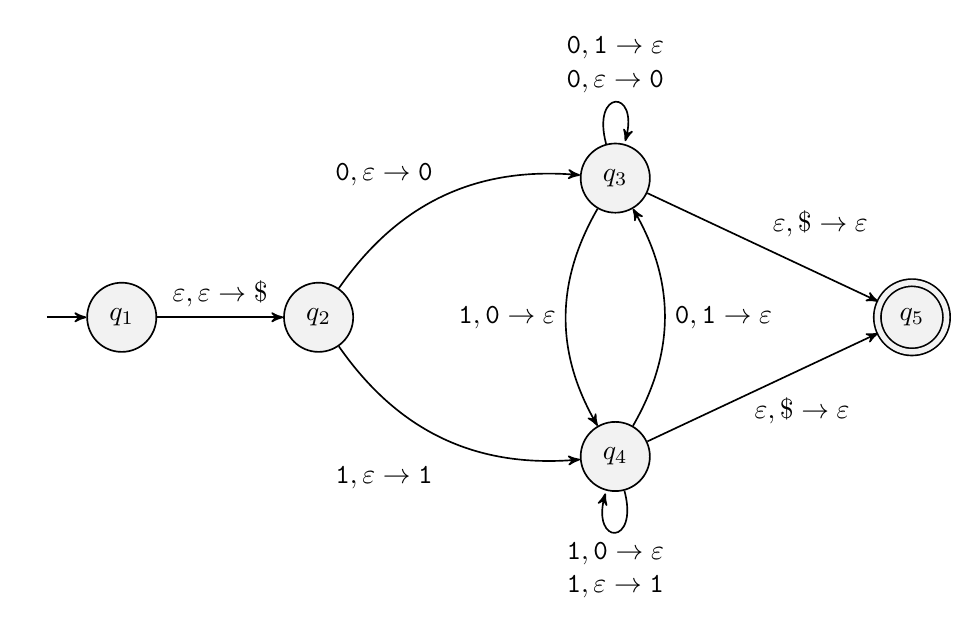
\begin{tikzpicture}
            \node[state, initial] (q1) {$q_1$};
            \node[state, right of = q1] (q2) {$q_2$};
            \node[state, above right of = q2, xshift=2cm] (q3) {$q_3$};
            \node[state, below right of = q2, xshift=2cm] (q4) {$q_4$};
            \node[state, above right of = q4, accepting, xshift=2cm] (q5) {$q_5$};

            \draw (q1) edge node {$\varepsilon, \varepsilon \rightarrow \$$} (q2);
            \draw (q2) edge[bend left] node {$ \texttt{0}, \varepsilon \rightarrow \texttt{0}$} (q3)
                edge[bend right, left] node[yshift=-0.5cm] {$\texttt{1}, \varepsilon \rightarrow \texttt{1}$} (q4);
            \draw(q3) edge[loop above] node[align=center] {$\texttt{0}, \texttt{1} \rightarrow \varepsilon$\\$\texttt{0}, \varepsilon \rightarrow \texttt{0}$} (q3)
                edge[bend right, left] node {$\texttt{1}, \texttt{0} \rightarrow \varepsilon$} (q4)
                edge node {$\varepsilon, \$ \rightarrow \varepsilon$} (q5);
            \draw (q4) edge[loop below] node[align=center] {$\texttt{1}, \texttt{0} \rightarrow \varepsilon$\\$\texttt{1}, \varepsilon \rightarrow \texttt{1}$} (q4)
                edge[bend right, right] node {$\texttt{0}, \texttt{1} \rightarrow \varepsilon$} (q3)
                edge[below] node[xshift=0.5cm] {$\varepsilon, \$ \rightarrow \varepsilon$} (q5);
        \end{tikzpicture}

        This automata describes the language $C$. The PDA's stack is used to keep track of the imbalance of \texttt{0}s and \texttt{1}s, and when a \texttt{0} or a \texttt{1} is read, if there is an opposiong \texttt{1} or \texttt{0} not on the stack, it itself is added to the stack. Otherwise, the opposing symbol is removed from the stack. Since you can only reach the accept state by popping a $\$$ from the stack, there must be an equal number of \texttt{0}s and \texttt{1}s in the string.

    \section{Language Complement}

        Prove the following language to be context-free by writing either a PDA \textit{or} a CFG for it:

        \begin{equation*}
            L_3 = \overline{\{\texttt{0}^n \texttt{1}^n \mid n \ge 0\}}
        \end{equation*}

        For example, \texttt{000111} $\notin L_3$. Hint: First prove that this is equal to $\{\texttt{0}^m \texttt{1}^n \mid m \neq n\} \cup \overline{\texttt{0}^* \texttt{1}^*}$. 

        $L_3$ covers two cases of $\{\texttt{0}, \texttt{1}\}^*$: 

        \begin{enumerate}[1.]
            \item The number of $\texttt{0}$s cannot be equal to the number of $\texttt{1}$s. Therefore, any string of the form $\texttt{0}^n \texttt{1}^n$ where $n \ge 0$ cannot be in the set.

            \item There must be at least one \texttt{0} following a \texttt{1}. Therefore, any string of the form $\texttt{0}^* \texttt{1}^*$ cannot be in the set.
        \end{enumerate}

        Using these characteristics, it is clear that $L_3$ = $\{\texttt{0}^m \texttt{1}^n \mid m \neq n\} \cup \overline{\texttt{0}^* \texttt{1}^*}$. 

        Seeing this, we can construct the grammar $G_3$ to generate strings that belong to $L_3$ with start state $S$:

        \begin{center}
        \begin{tabular}{ll}
            $S \longrightarrow Z \mid O \mid P$ \\
            $Z \longrightarrow \texttt{0}Z \mid \texttt{0}A$ \\
            $A \longrightarrow \texttt{0}A\texttt{1} \mid \varepsilon$ \\
            $O \longrightarrow O\texttt{1} \mid B\texttt{1}$ \\
            $B \longrightarrow \texttt{0}B\texttt{1} \mid \varepsilon$ \\
            $P \longrightarrow C\texttt{10}C$ \\
            $C \longrightarrow \texttt{0}C \mid C\texttt{1} \mid \varepsilon$
        \end{tabular}
        \end{center}

        The $Z$ rule is to ensure there are always more \texttt{0}s than \texttt{1}s. By forcing the extra \texttt{0}s, whatever result is generated by the $Z$ rule will be in $L_3$.

        The $O$ rule is to ensure there are always more \texttt{1}s than \texttt{0}s. By forcing the extra \texttt{1}s, whatever result is generated by the $O$ rule will be in $L_3$.

        The $P$ rule is to ensure a \texttt{0} will always follow at least one \texttt{1}. Covering this case, the generated string will be a member of $\overline{\texttt{0}^* \texttt{1}^*}$, and therefore a member of $L_3$






    
\end{document}
